\documentclass{report}
\usepackage[utf8]{inputenc}
\usepackage{amssymb}
\usepackage{amsmath}
\usepackage{hyperref}
\usepackage{tcolorbox}
\tcbuselibrary{theorems}

% Things I use, but too lazy to find how again

%%%%%%%%%%%%%%%%%%%%%%%%%%%%%%%%%%%%%%%%%%%%%%%%%%%%
% Make a hyperlink to another section:
% \hyperref[sec:hello]{Word of text} (set link to hello)

% \section{Hello World} 
% \label{sec:hello} (define a label for the section
%%%%%%%%%%%%%%%%%%%%%%%%%%%%%%%%%%%%%%%%%%%%%%%%%%%%
% Make an unordered list:
% \begin{itemize}
%   \item 
%   \item
% \end{itemize}
%%%%%%%%%%%%%%%%%%%%%%%%%%%%%%%%%%%%%%%%%%%%%%%%%%%%
% Make an ordered list:
% \begin{enumerate}
%   \item 
%   \item
% \end{itemize}
%%%%%%%%%%%%%%%%%%%%%%%%%%%%%%%%%%%%%%%%%%%%%%%%%%%%
% Make a matrix
%\begin{bmatrix}
%        x_1y_1 & x_1y_2 & \dots  & x_1y_m \\
%        x_2y_1 & x_2y_2 & \dots  & x_2y_m \\
%        \vdots & \vdots & \ddots & \vdots \\
%        x_ny_1 & a_{m2} & \dots  & x_ny_m \\
%   \end{bmatrix}
%%%%%%%%%%%%%%%%%%%%%%%%%%%%%%%%%%%%%%%%%%%%%%%%%%%%
% Make an equation:
% \begin{equation}
% ...
% \end{equation}
%%%%%%%%%%%%%%%%%%%%%%%%%%%%%%%%%%%%%%%%%%%%%%%%%%%%
% Theorems:
%\begin{mytheo}{Title}{NameOfTheorem}
% ...
%\end{mytheo}
%%%%%%%%%%%%%%%%%%%%%%%%%%%%%%%%%%%%%%%%%%%%%%%%%%%%
% N'th order linear equation
% $$y^{(n)}(t) + ... + p_1(t)y'(t) + p_0(t)y(t) = 0$$
%%%%%%%%%%%%%%%%%%%%%%%%%%%%%%%%%%%%%%%%%%%%%%%%%%%%

\newtcbtheorem[number within=section]{mytheo}{Theorem}
{colback=orange!5,colframe=red!35!black,fonttitle=\bfseries}{th}

\hypersetup{
    pdftitle={Thermodynamics},
    pdfpagemode=FullScreen,
}




\title{Theromodynamics}
\author{Arun Khanna}
\date{}

\begin{document}

\maketitle
\tableofcontents

\newpage

\chapter{Zeroth Law and Thermal Expansion}
\section{Definitions}

Let's begin with some definitions (yay!):

\begin{itemize}
	\item \textbf{Internal Energy} is the energy of a system composed of the sum of all the energy in the molecules that consist the system in a system when looked at from the center of mass frame. It is composed of two parts, \textbf{thermal energy} (kinetic energy of molecules) and \textbf{bond energy} (potential energy of bonds).
	\item \textbf{Thermal Energy} is the part of the internal energy of a body associated with the random movement (kinetic energy) of the molecules.
	\item \textbf{Temperature} is a measure of the average thermal energy of each molecule in a body.
	\item \textbf{Heat} is the transfer of energy from one body to another due to a temperature difference.
	\item \textbf{Thermal Contact} between two bodies occurs when it is possible for heat to be transferred in between them.
	\item \textbf{Thermal Equilibrium} occurs between two objects when the two objects are placed together and there is no transfer of energy due to heat or electromagnetic radiation.
	
\end{itemize}

We can think about temperature as a measure of the internal energy of some body (a measure of how much the molecules within it "vibrate").

Thus, when we put a body with higher temperature $B_1$ (higher thermal energy) next to a body with a lower temperature $B_2$, we expect the faster moving molecules
to impart momentum onto the molecules of the slower moving molecules in $B_2$. 

After this process occurs, we notice that $B_1$ now has a lower temperature than before and $B_2$ has a higher temperature.




\section{Zeroth Law of Thermodynamics}

The definitions above can help us define the Zeroth Law of Thermodynamics:

\begin{mytheo}{Zeroth Law of Thermodynamics}{zeroth}
	If two bodies A and B are in thermal equilibrium with a third object C, then A and B are in thermal equilibrium with one another 
\end{mytheo}

This, in hindsight, might seem obvious, but it is important since it allows us to measure the average thermal energy of an object relative to other objects with the same average thermal energy.

In fact, when two bodies are in thermal equilibrium, they also must have the same temperature! Thus, we can say that all bodies that can be placed at thermal equilibrium have the same temperature.



\section{Temperature Scales}
There are different scales we can measure temperature with:

Celsius is the most common scale in the world. Zero degrees celsius is defined to be the temperature at which gaseous, liquid and solid water can coexist simultaneously (triple point). 100 degrees is the point at which water boils at atmospheric pressure.

It turns out that at a constant volume, a temperature change for a gas produces an approximately linear change in pressure. We can measure this using an apparatus like shown below:

\begin{center}
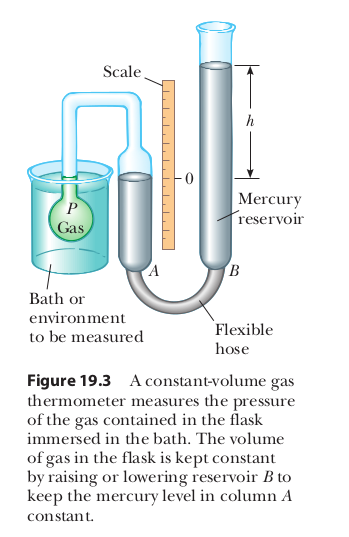
\includegraphics[scale=0.5]{temp_pres.png}
\end{center}


We can use this to find the linear relationship and the slope of the line. If we extrapolate the line to a pressure of 0, we see that the temperature will be around $-273.16$ degrees Celsius. This is true for different gases:


\begin{center}
	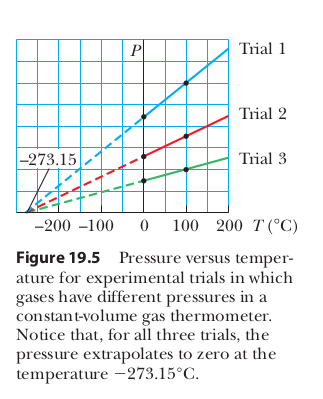
\includegraphics[scale=0.5]{temp_intepolate.png}
\end{center}


We can define a new scale based on this point. We define \textbf{absolute zero} where the temperature of a gas at constant pressure has an arbitrarily small pressure. We call this scale the \textbf{Kelvin scale}.

In addition, we made the value $273.16 K$ the triple point of water. This is so it would be easy to convert between this new absolute scale and the celsius scale:

$$T_K = T_C + 273.16 $$ 

In addition, there is the \textbf{Fahrenheit} scale used in the United States where the freezing point of water is $32$ and the boiling point is $212$

We know that the change in temperature from Fahrenheit will be the same as the change in temperature in Celsius, so:

$$(212-32)F = (100-0)C$$

$$1 C = \frac{9}{5}F$$

Thus one degrees Fahrenheit can be directly converted into Celsius and vice-versa.

Since we know that the freezing point of water is 0 degrees Celsius and 32 degrees Fahrenheit:
$$T_C = \frac{9}{5}T_F + 32$$


\section{One-Dimensional Expansion}

When there is a transfer in energy due to heat into an object, it usually expands.

Microscopically, at room temperature, molecules oscillate around their equilibrium point around $10^{-11} m$ and with a frequency of $10^{13}$ Hz. The spacing is around $10^{-10}$ m (so the spacing is smaller than the actual amplitude). Since when we heat the molecules the amplitude increases, usually creating a greater spacing in between them. 

If the expansion is small relative to the initial length, we can approximate the change in length as proportional to the change in temperature.

Thus:

$$
\boxed{
\Delta L = \alpha L_i \Delta T
}
$$

$$L_f = (1+\alpha\Delta T)L_i$$

Note that for some materials, $\alpha$ may be small for some dimensions because of the chemical structure of that material.


\section{Volumetric Expansion}
Let's assume we have a material that is \textbf{isotropic}, that is the coefficient of linear expansion is the same in all dimensions.

Let's consider a box with initial dimensions $l_i, w_i, h_i$. Since, we expect expansion in all dimensions:

$$l_f = (1+\alpha\Delta T)l_i$$
$$w_f = (1+\alpha\Delta T)w_i$$
$$h_f = (1+\alpha\Delta T)h_i$$


We know that the initial volume is $V = lwh$. Therefore, the new volume is:

$$V_f = l_fw_fh_f$$ 
$$= [(1+\alpha\Delta T)l_i][(1+\alpha\Delta T)w_i][](1+\alpha\Delta T)h_i]$$ 
$$= (1+\alpha\Delta T)^3l_iw_ih_i$$
$$V_f = (1+\alpha\Delta T)^3V_i$$

We know from the binomial theorem, that we can expand the cubic term out to:

$$V_f =  [1+3\alpha\Delta T + 3(\alpha\Delta T)^2 + (\alpha\Delta T)^3]V_i$$

The value of $\alpha$ is usually really small (on the order of $10^{-5}$). Thus, when we square and cube it, it will almost equal 0:

$$V_f \approx  (1+3\alpha\Delta T)V_i$$

This looks awfully lot like our expansion in one dimension formula.If we define:

$$\beta = 3\alpha$$

as our coefficient of volumetric expansion, we get:

$$V_f \approx  (1+\beta\Delta T)V_i$$

\section{Volumetric Expansion of Gases}








\chapter{First Law of Thermodynamics}
\section{Work and Heat}
\section{PV Diagrams}
\section{Types of Thermodynamic Processes}
\section{Methods of Heat Transfer}




\chapter{Questions}
\begin{itemize}
    \item From a microscopic level, why does a hole grow during thermal expansion?
\end{itemize}

\newpage



\end{document}
